%%%%%%%%%%%%%%%%%%%%%%%%%%%%%%%%%%%%%%%%%
% University/School Laboratory Report
% LaTeX Template
% Version 3.1 (25/3/14)
%
% This template has been downloaded from:
% http://www.LaTeXTemplates.com
%
% Original author:
% Linux and Unix Users Group at Virginia Tech Wiki 
% (https://vtluug.org/wiki/Example_LaTeX_chem_lab_report)
%
% License:
% CC BY-NC-SA 3.0 (http://creativecommons.org/licenses/by-nc-sa/3.0/)
%
%%%%%%%%%%%%%%%%%%%%%%%%%%%%%%%%%%%%%%%%%

%----------------------------------------------------------------------------------------
%	PACKAGES AND DOCUMENT CONFIGURATIONS
%----------------------------------------------------------------------------------------

\documentclass{article}
\usepackage{hyperref}
\usepackage[utf8]{inputenc}
\usepackage[italian]{babel} 
\usepackage[version=3]{mhchem} % Package for chemical equation typesetting
\usepackage{siunitx} % Provides the \SI{}{} and \si{} command for typesetting SI units
\usepackage{graphicx} % Required for the inclusion of images
\usepackage{natbib} % Required to change bibliography style to APA
\usepackage{amsmath} % Required for some math elements 
\usepackage{csvsimple}
\usepackage{adjustbox}
\usepackage{longtable}
\usepackage{booktabs}
\usepackage{color}
\usepackage{accsupp}
\usepackage{listings}
\usepackage{setspace}
\usepackage{graphicx} 
\definecolor{Code}{rgb}{0,0,0}
\definecolor{Decorators}{rgb}{0.5,0.5,0.5}
\definecolor{Numbers}{rgb}{0.5,0,0}
\definecolor{MatchingBrackets}{rgb}{0.25,0.5,0.5}
\definecolor{Keywords}{rgb}{0,0,1}
\definecolor{self}{rgb}{0,0,0}
\definecolor{Strings}{rgb}{0,0.63,0}
\definecolor{Comments}{rgb}{0,0.63,1}
\definecolor{Backquotes}{rgb}{0,0,0}
\definecolor{Classname}{rgb}{0,0,0}
\definecolor{FunctionName}{rgb}{0,0,0}
\definecolor{Operators}{rgb}{0,0,0}
\definecolor{Background}{rgb}{0.98,0.98,0.98}
\lstdefinestyle{java}{
  belowcaptionskip=1\baselineskip,
  breakatwhitespace=false,        % sets if automatic breaks should only happen at whitespace
  breaklines=true,                % sets automatic line breaking
  xleftmargin=\parindent,
  language=Java,
  tabsize=4, 
  tabsize=4,
  numbers=left,
  showstringspaces=false,
  basicstyle=\footnotesize\ttfamily,
  keywordstyle=\bfseries\color{blue},
  commentstyle=\itshape\color{blue},
  frame=single],
  resetmargins=true,
}
\lstdefinelanguage{Python}{
numbers=left,
numberstyle=\footnotesize,
numbersep=1em,
xleftmargin=1em,
framextopmargin=2em,
framexbottommargin=2em,
showspaces=false,
showtabs=false,
showstringspaces=false,
frame=l,
tabsize=4,
% Basic
basicstyle=\ttfamily\small\setstretch{1},
backgroundcolor=\color{Background},
% Comments
commentstyle=\color{Comments}\slshape,
% Strings
stringstyle=\color{Strings},
morecomment=[s][\color{Strings}]{"""}{"""},
morecomment=[s][\color{Strings}]{'''}{'''},
% keywords
morekeywords={import,from,class,def,for,while,if,is,in,elif,else,not,and,or,print,break,continue,return,True,False,None,access,as,,del,except,exec,finally,global,import,lambda,pass,print,raise,try,assert},
keywordstyle={\color{Keywords}\bfseries},
% additional keywords
morekeywords={[2]@invariant,pylab,numpy,np,scipy},
keywordstyle={[2]\color{Decorators}\slshape},
emph={self},
emphstyle={\color{self}\slshape},
%
}
\setlength\parindent{0pt} % Removes all indentation from paragraphs

\renewcommand{\labelenumi}{\alph{enumi}.} % Make numbering in the enumerate environment by letter rather than number (e.g. section 6)

% CSV import

%\usepackage{times} % Uncomment to use the Times New Roman font

%----------------------------------------------------------------------------------------
%	DOCUMENT INFORMATION
%----------------------------------------------------------------------------------------

\title{Simulazione di un supermercato con Anylogic} % Title

\author{Odore Marco} % Author name

\date{\today} % Date for the report

\begin{document}

\maketitle % Insert the title, author and date

\begin{center}
\begin{tabular}{l l}

Docenti: & Trubian Marco, Malchiodi Dario\\% Instructor/supervisor
Corso: & Simulazione e Teoria delle code
\end{tabular}
\end{center}

\tableofcontents
% If you wish to include an abstract, uncomment the lines below
% \begin{abstract}
% Abstract text
% \end{abstract}

%----------------------------------------------------------------------------------------
%	SECTION 1
%----------------------------------------------------------------------------------------

\section{Scopo del progetto}

L'obiettivo del progetto è quello di simulare, tramite il software Anylogic\footnote{\url{https://www.anylogic.com/}}, diverse dinamiche riguardanti un supermercato, come ad esempio il flusso della clientela, la schedulazione del personale e i diversi servizi che possono essere presenti nell'attività. 
\newline
\newline
Il tutto è realizzato tramite la versione \emph{learning edition} del software, che presenta alcune limitazioni, come ad esempio il numero massimo di tipologie definibili per gli agenti e un numero massimo per la loro generazione durante l'esecuzione della simulazione\footnote{Durante la simulazione saranno generabili un massimo di 50000 agenti complessivi e in fase di costruzione del modello non è stato possibile definire più di 10 agenti.}.

\section{Agent Based modeling}
Data la natura complessa del problema, che possiede moltissime attività parallele e concorrenti da simulare, si è deciso di sfruttare il modello basato su agenti.
\newline
\newline
Nello specifico sono definiti i seguenti agenti:
\begin{itemize}
\item \textsf{Customer}:  il cliente del supermercato.
\item \textsf{Worker}:  i diversi addetti dei reparti di panetteria, pescheria e macelleria.
\item \textsf{Warehouseman}: i magazzinieri che si occupano di rifornire gli scaffali.
\item \textsf{Cashier}: i cassieri per il servizio di pagamento.
\item \textsf{Cart}: i carrelli utilizzati dai clienti.
\item \textsf{GenericFood}: la risorsa utilizzata dai magazzinieri per rifornire gli scaffali.
\item \textsf{AutomaticCashierMachine}: la cassa automatica per il servizio di pagamento.
\item \textsf{InfoPointHelper}: gli addetti dell'info point.
\end{itemize}

La maggior parte degli agenti è definita per poterne differenziare l'aspetto all'interno della simulazione, e solo \textsf{Customer} e \textsf{GenericFood} possiedono un'ulteriore caratterizzazione.
\subsection{Gli agenti Customer e genericFood}
Il \textsf{Customer} possiede diverse variabili e parametri. Nello specifico:
\begin{itemize}
\item Variabile \textsf{ItemsToBuy}: È un dizionario con coppie Prodotto(String)/Quantità(int), che contiene i prodotti che il cliente vuole comprare e relativa quantità.
\item Variabile \textsf{Bought}: Un booleano che indica se il cliente ha comprato qualcosa, inizializzato a false.
\item Variabile \textsf{CounterBuy}: un contatore(int) che indica quanti prodotti il cliente ha nel carrello in quel momento.
\item Variabile \textsf{NeedsInfo}: Un booleano che indica se il cliente necessita di chiedere informazioni all'infopoint.
\item I parametri \textsf{needsInfoRate}, \textsf{needsMeat}, \textsf{needsBread}, \textsf{needsFish}, \textsf{needsOther}: che rappresentano le diverse probabilità di acquisto (o di richiesta info) che un cliente generico possiede entrando nel supermercato\footnote{Ad esempio, nella simulazione è stata definita la probabilità che un cliente  voglia comprare del pane entrando nel supermercato a 0.7(cioè sette clienti su dieci).}.
\end{itemize}
L'agente è inoltre caratterizzato da uno state chart (Figura 1), con tre diversi stati:
\begin{itemize}
\item \textsf{InitialState}: lo stato iniziale del cliente entrando nel supermercato.
\item \textsf{WantsToBuy}: lo stato del cliente quando è in fase di acquisto dei prodotti.
\item \textsf{WantsToGoAway}: lo stato finale del cliente, quando decide di lasciare il supermercato.
\end{itemize}

\begin{center}
\begin{figure}[h]
\center
\label{statechart}
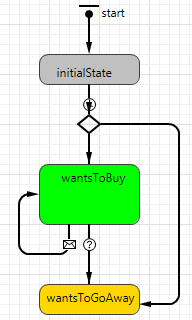
\includegraphics[scale=0.47]{./statechart.png}
\caption{\footnotesize{Il diagramma di stato dell'agente Customer.}}
\end{figure}
\end{center}
Quando il cliente entra nello stato InitialState, viene eseguito del codice (Figura 2) che permette di inizializzare la variabile ItemsToBuy di Customer, sfruttando i diversi parametri descritti in precedenza che definiscono le probabilità di acquisto del cliente per i diversi prodotti.
\newline
\newline
Una volta inizializzata la lista della spesa, se questa è vuota il Customer passerà allo stato WantsToGoAway, altrimenti entrerà nello stato loop WantsToBuy, finché non avrà collezionato tutti gli oggetti, per poi finire anch'esso nello stato finale WantsToGoAway.
\begin{center}
\begin{figure}[h]
\label{init}
\lstinputlisting[style=java]{./init.java}
\caption{\footnotesize{Inizialmente viene eseguito uno shuffle sulla lista di stringhe dei possibili oggetti da acquistare, per differenziare l'ordine di acquisto di ogni cliente, e poi viene simulata un'estrazione da una distribuzione di Bernoulli sfruttando una distribuzione uniforme e il parametro del prodotto di riferimento. Viene inoltre simulata l'estrazione da una distribuzione uniforme discreta (da 1 a 4 oggetti) per la quantità del prodotto da acquistare. Il metodo \textsf{getParamaterFromString} è una ulteriore funzione custom, definita per il recupero dei valori dei parametri.}}
\end{figure}
\end{center}
Per quanto riguarda l'agente \textsf{genericFood}, questo possiede due attributi per caratterizzarlo, ovvero:
\begin{itemize}
\item \textsf{Type}: Di tipo String. Specifica la tipologia di prodotto (Es. "meat").
\item \textsf{Quantity}: Di tipo Int. Specifica la quantità di prodotto da acquistare.
\end{itemize}

\section{Il supermercato e i servizi}
Il supermercato si estende su una superfice rettangolare, con l'area centrale dedicata agli scaffali per i prodotti generici, la parte destra ai servizi al banco, la parte inferiore ai servizi di cassa, e i magazzini disposti sia sul lato superiore (2) che sul lato sinistro (1). Nella figura 3 è mostrata la planimetria del supermercato e le sue principali aree di interesse.
\begin{center}
\begin{figure}[h]
\center
\label{planim}
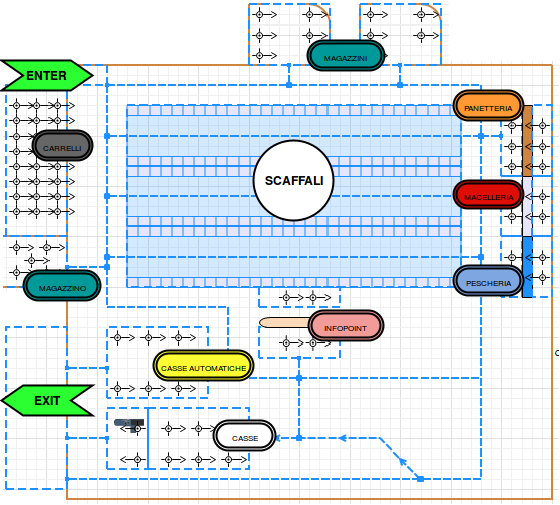
\includegraphics[scale=0.5]{./planimetria1.png}
\caption{\footnotesize{Le principali aree di interesse del supermercato.}}
\end{figure}
\end{center}
Ognuno dei servizi implementati possiede un numero variabile di risorse (rappresentate dagli agenti), che vengono schedulate in base all'orario del giorno (ad eccezione delle casse automatiche). Nello specifico abbiamo:
\begin{itemize}
\item Servizio al banco per prodotti di panetteria (agenti Worker).
\item Servizio al banco per prodotti di macelleria (agenti Worker).
\item Servizio al banco per prodotti di pescheria (agenti Worker).
\item Servizio di infopoint (agenti InfoPointHelper).
\item Servizio di pagamento con cassiere (agenti Cashier).
\item Servizio di pagamento con cassa automatica (agenti AutomaticCashierMachine).
\end{itemize}
Oltre ai servizi alla clientela sono simulate anche delle attività di rifornimento degli scaffali (agenti WarehouseWorker) per tre diverse tipologie di prodotti (agenti GenericFood), che per comodità, e a causa delle limitazioni della versione learning di anylogic, si differenziano unicamente per il colore (verde, viola, giallo).
\section{Flow Diagrams}
Per caratterizzare il comportamento dei clienti (agente Customer) e dei prodotti generici da scaffale (genericFood) all'interno del supermercato, sono definiti 4 diagrammi di flusso, di cui 3 dedicati alle tre diverse tipologie di prodotti.
\subsection{Customer Flow}
I tempi di arrivo (e generazione) dell'agente Customer nel supermercato sono definiti nel flow (Figura 4) all'interno di un blocco sorgente, chiamato \textsf{customerSource}, grazie ad uno scheduling temporale sulle 24 ore. Ogni ora del giorno ha infatti un \textit{rate}\footnote{Parametro di una distribuzione esponenziale, con media $\frac{1}{rate} $ } di arrivo specifico. Questo ha permesso di simulare il diverso flusso di clientela che caratterizza la giornata di un supermercato, modulando ad esempio su frequenze più basse gli arrivi notturni, per poi aumentarle durante il giorno (con dei picchi nelle ore di punta).
\newline
\newline
Il percorso che il Customer seguirà all'interno del flow diagram (e quindi all'interno del supermercato) è definito dal suo stato interno corrente e quindi dal valore delle sue variabili (itemsToBuy, Bought, etc). Il cliente potrà ad esempio decidere se prendere un carrello (se deve comprare più di 10 oggetti), recuperare un prodotto dagli scaffali o dai reparti da banco, pagare alla cassa automatica (se ha meno di 10 oggetti) o a quella con cassieri, se chiedere info all'InfoPoint o , se non deve acquistare nulla, uscire direttamente dal supermercato.

\begin{center}
\begin{figure}[h]
\center
\label{custflow}
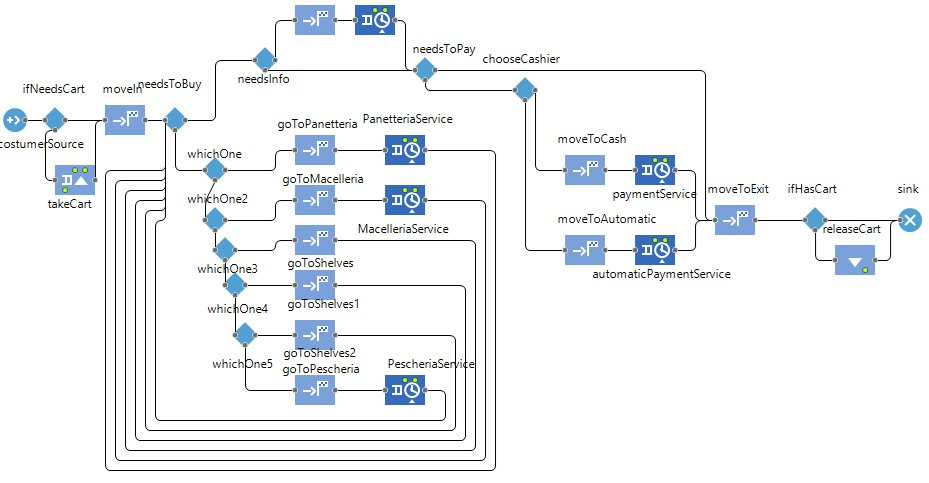
\includegraphics[scale=0.5]{./cust_flow.jpg}
\caption{\footnotesize{Lo schema di flusso del customer nel supermercato.}}
\end{figure}
\end{center}

\subsection{GenericFood flow}
Anche i tempi di arrivo degli agenti genericFood sono regolati da uno scheduling orario (come sempre specificato nel nodo sorgente), che tenta di simulare il rifornimento dei magazzini e degli scaffali. Essendoci tre tipologie per questo agente, sono definiti tre flow corrispondenti (Figura 5).

\begin{center}
\begin{figure}[h]
\center
\label{foodflow}
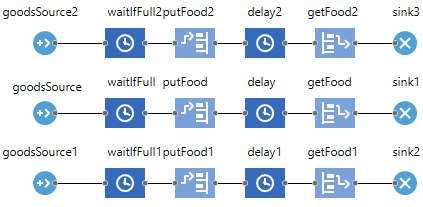
\includegraphics[scale=0.5]{./food_flow.jpeg}
\caption{\footnotesize{Lo schema di flusso del genericFood nel supermercato.}}
\end{figure}
\end{center}
Il movimento all'interno del supermercato degli agenti genericFood dipende fortemente dalle risorse e dagli agenti che vi interagiscono. Lo spostamento del prodotto sugli scaffali è infatti vincolato alla turnazione dei magazzinieri\footnote{\footnotesize{Gli agenti/risorse warehouseWorker spostano gli agenti genericFood tramite il nodo RackStore (chiamato \textsf{putFood} nel flow), ma solo se gli scaffali non sono pieni (nodo \textsf{waitIfFull}).}}. Quando poi un cliente vuole recuperare uno dei prodotti, lo "sblocca"\footnote{\footnotesize{Il singolo agente genericFood viene rilasciato dallo scaffale (nodo \textsf{getFood}) ed eliminato (nodo \textsf{Sink} nel flow)}} dopo la chiamata di una funzione di \textsf{stopDelay} (riferita al nodo \textsf{Delay} nel flow), per poi poterlo acquistare\footnote{\footnotesize{Non è stata gestita la quantità di prodotto richiesta dal singolo Customer, nè la situazione in cui lo scaffale non contiene il prodotto richiesto. Di fatto per il Customer il prodotto sarà considerato recuperato a prescindere dalla quantità e dalla sua disponibilità.}}.

\section{Statistiche e diagrammi}
Si sono realizzati diversi diagrammi (Figura 6) per ricavare informazioni dalla simulazione, nello specifico:
\begin{itemize}
\item Istogramma che mostra le proporzioni totali di utilizzo delle casse automatiche e casse con cassieri. Si basa su delle variabili globali (\textsf{totBuy} e \textsf{totBuyAut}) che tengono traccia dell'utilizzo delle casse.
\item Grafico a torta che mostra le proporzioni totali dei prodotti acquistati nel supermercato (pane, carne, pesce, prodotti generici), che si basa sulla variabile globale \textsf{countProducts}.
\item Grafico che mostra la lunghezza delle diverse code dei servizi presenti nel supermercato, al tempo corrente.
\item Istogrammi per le frequenze di arrivo orario per l'agente Customer e per l'agente genericFood. Si basano sugli Histogram Data \textsf{ArrivalRate} e \textsf{ArrivalFoodRate}, che vengono aggiornati nei nodi sorgente, con la funzione \textsf{getHourOfDay}.
\end{itemize}
\begin{center}
\begin{figure}[h]
\center
\label{diagrams}
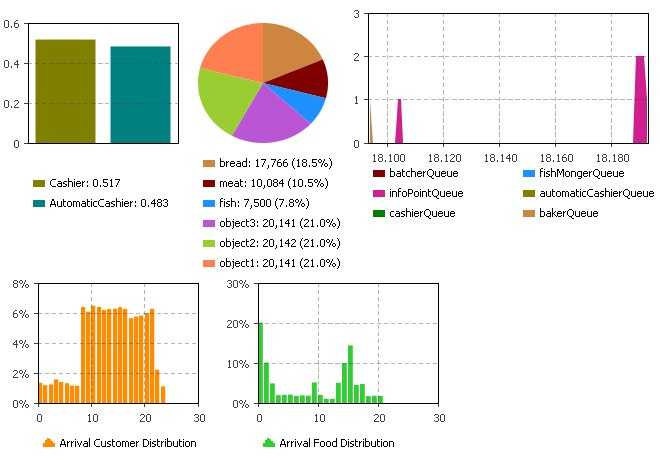
\includegraphics[scale=0.6]{./diagrams.jpeg}
\caption{\footnotesize{Statistiche sull'esecuzione di una simulazione fino a 50.000 agenti.}}
\end{figure}
\end{center}

\section{Lavori futuri}
Esistono diversi scenari di espansione del progetto:
\begin{itemize}
\item L'aggiunta di un servizio rifornimento magazzini con l'arrivo di camion, schedulati anch'essi con un rate orario.
\item L'aggiunta di diagrammi per i tempi di attesa dei servizi, per la loro ottimizzazione.
\item La simulazione dell'impazienza del Customer per un'eventuale attesa troppo lunga.
\item La gestione del quantitativo dei prodotti da scaffale e la produzione dei prodotti da banco. 
\item La simulazione di un incendio/emergenza per la verifica delle vie di fuga. 
\item L'introduzione di un parcheggio per la clientela (e sua gestione).
\end{itemize}
\end{document} 